\documentclass[journal]{IEEEtran}

\usepackage{cite}
\usepackage{amsmath,amssymb,amsfonts}
\usepackage{algorithmic}
\usepackage{graphicx}
\usepackage{textcomp}
\usepackage{hyperref}
\usepackage{xcolor}
\usepackage{array}
\usepackage{tcolorbox}
\usepackage{fancyhdr}

% Add the header for the report
\pagestyle{fancy}
\fancyhf{}
\fancyhead[C]{BIM453 Introduction to Machine Learning Term Project - 2024-2025 Fall}

\def\BibTeX{{
    \rm B\kern-.05em{\sc i\kern-.025em b}\kern-.08em
    T\kern-.1667em\lower.7ex\hbox{E}\kern-.125emX
}}

\begin{document}

\title{[Lung Disease Classification from Chest X-Rays]}

\author{
    \IEEEauthorblockN{
    \flushleft Emre Dumbo, 99990935744}
    
    \IEEEauthorblockA{
    \flushleft \textit{Department of Computer Engineering}, emredumbo@ogr.eskisehir.edu.tr}
    
    \vspace{1.5mm} % Adjust vertical spacing as needed
    
    \IEEEauthorblockN{
    \flushleft Buğra Muhçi, 14492562250}
    
    \IEEEauthorblockA{
    \flushleft \textit{Department of Computer Engineering}, bugramuhci@ogr.eskisehir.edu.tr}
}



\maketitle

% Ensure the header appears on the first page
\thispagestyle{fancy}

\begin{abstract}  
This project focuses on the classification of grayscale images into 6 categories using deep learning techniques. Initially, the NIH Chest X-rays dataset \cite{nih-chest-xrays} \cite{google-drive} contained 112,000 images across 14 classes. Through a cleaning and preprocessing process, this dataset was reduced to 19,561 images, narrowing down the focus to 6 important categories. A custom deep learning pipeline using the ResNet50\cite{keras-api} \cite{google-drive} architecture was developed to preprocess, augment, and train the model. The preprocessing steps included normalizing grayscale images and using class weight balancing to address the issue of data imbalance. In addition, techniques like label smoothing and dynamic learning rate scheduling were applied to improve model performance. The final model achieved a validation accuracy of 55\%, demonstrating its capability in real-world classification tasks. This project highlights skills in machine learning, model optimization, and the importance of efficient data preparation to achieve meaningful results.
\end{abstract}


\begin{IEEEkeywords}
Machine learning, deep learning, image classification, grayscale image processing, ResNet50, class imbalance, data preprocessing, TensorFlow, accuracy.
\end{IEEEkeywords}

% Commented out the Project Proposal part
% \section{Project Proposal}
% The project proposal is the initial document that outlines the main objectives, methodology, and project members of your project. It should be brief, not exceeding 1 page, and must include:
% \begin{itemize}
%     \item \textbf{Project Title:} A descriptive title that summarizes the core of your project.
%     \item \textbf{Project Members:} List the full names and student IDs of all group members.
%     \item \textbf{Problem Statement:} A brief description of the problem you are addressing and why it is significant.
%     \item \textbf{Proposed Methodology:} Outline the methods and machine learning models you plan to use for solving the problem.
%     \item \textbf{Dataset Description:} Provide a brief overview of the dataset you will use, including the source, number of instances, and key features.
% \end{itemize}
% The project proposal should be submitted by the given deadline and will constitute 20\% of the final grade.

\section{Introduction}

Lung diseases such as pneumothorax and atelectasis are significant health challenges worldwide \cite{med-student-koroglu}. Chest X-rays are commonly used for diagnosing these conditions, but interpreting them requires specialized knowledge, which is not always available, especially in areas with limited resources \cite{dr-kazazi}. Machine learning has emerged as a potential solution to automate this process, offering faster and more accurate diagnoses.

In this project, the goal was to classify lung diseases from chest X-rays using 4 different machine learning models: MobileNetV3, EfficientNet, ResNet50, and a custom Convolutional Neural Network (CNN) \cite{keras-api}. Among these, ResNet50 yielded the best validation accuracy, demonstrating its effectiveness for this task. This study provided practical experience with machine learning techniques and insights into how variations in model architecture and training strategies impact performance.

The dataset and the trained ResNet50 Model used in this study is accessible via Google Drive at \href{https://drive.google.com/drive/folders/1DMyWrGlT2p1CiQlM6K2aXYlUdI-efoyM?usp=sharing}{this link} \cite{google-drive}.



\section{Proposed Methodology}
In this project, we aim to classify grayscale images into 6 categories using machine learning techniques, focusing on image classification tasks. The methodology consists of 4 main components: model selection, implementation strategy, evaluation metrics, and testing setup.

\subsection{Model Selection}
We used \textbf{ResNet50}, a deep convolutional neural network (CNN) architecture known for its residual connections, which help mitigate the vanishing gradient problem and allow for deeper learning. ResNet50 has been successfully applied in various image classification tasks, making it an ideal choice for our problem. Additionally, we leveraged \textbf{transfer learning}, utilizing a pre-trained ResNet50 model on ImageNet to benefit from learned features, thus reducing the need for extensive training time and computational resources.

\subsection{Implementation Strategy}
The first step involved data preprocessing. Grayscale images were converted to RGB format to match the input requirements of ResNet50. The images were resized to 224x224 pixels, normalized, and augmented using techniques such as random rotations, zooms, and shifts \cite{prof-candemir}. This augmentation enhanced the generalization ability of the model and prevented overfitting. The ResNet50 model was fine-tuned by removing its top layers and adding custom layers specific to our 6-class classification task. These layers included a \textbf{Global Average Pooling} layer, a \textbf{dropout} layer for regularization, and a \textbf{dense} layer with a \textbf{softmax} activation function to predict class probabilities \cite{prof-koc} \cite{prof-candemir} \cite{prof-karahoda}. 

\subsection{Evaluation Metrics}
The model's performance was primarily evaluated using \textbf{accuracy}, which indicates the proportion of correct predictions. To assess the model’s ability to differentiate between classes, we also used \textbf{AUC (Area Under the Curve)}. Additionally, considering potential class imbalances, we evaluated the model using \textbf{precision}, \textbf{recall}, and \textbf{F1-score}. These metrics provided a more comprehensive understanding of the model's performance in various class distribution scenarios, ensuring that each class was handled appropriately.

\subsection{Testing Setup}
The project was implemented in \textbf{Python} \cite{python} using \textbf{TensorFlow} and \textbf{Keras}\cite{tensorflow} as the machine learning frameworks. The model was trained on a system equipped with an \textbf{NVIDIA GeForce RTX 3060 Laptop GPU}, providing 3472 MB of memory, ensuring faster processing for training. The training environment was managed through \textbf{Anaconda} in a Python 3.10 environment \cite{anaconda}. The dataset was stored locally, with separate directories for the training, validation and test sets. The validation set was used to assess the model’s generalization ability and prevent overfitting.

This methodology combined pre-trained models with robust data preprocessing, class-weight balancing, and careful evaluation metrics to efficiently and accurately classify grayscale images into 6 categories. Through this approach, we demonstrated the effectiveness of deep learning for real-world image classification tasks.

\section{Experiments and Results}
In this section, we present the results of our lung disease classification experiments. The performance of the ResNet50 model was evaluated using multiple metrics, as shown in Table~\ref{tab:metrics}. Table~\ref{tab:class_metrics} provides class-wise sensitivity and specificity, which are critical in medical projects. Additionally, Figure~\ref{fig:roc_curve} illustrates the ROC-AUC curve for the classification task, with the reference to it explained below the image.

\subsection{Performance Metrics}

\begin{table}[h!]
    \centering
    \caption{Performance Metrics for ResNet50 Model}
    \label{tab:metrics}
    \begin{tabular}{|l|c|}
        \hline
        \textbf{Metric} & \textbf{Value} \\
        \hline
        Accuracy & 0.55 \\
        Precision (Macro) & 0.56 \\
        Precision (Weighted) & 0.58 \\
        Recall (Macro) & 0.61 \\
        Recall (Weighted) & 0.55 \\
        F1 Score (Macro) & 0.56 \\
        F1 Score (Weighted) & 0.55 \\
        ROC-AUC (One-vs-Rest, Macro) & 0.87 \\
        Balanced Accuracy & 0.55 \\
        \hline
    \end{tabular}
\end{table}

\subsection{Class-Wise Metrics}

\begin{table}[h!]
    \centering
    \caption{Class-Wise Sensitivity and Specificity}
    \label{tab:class_metrics}
    \begin{tabular}{|l|c|c|}
        \hline
        \textbf{Class} & \textbf{Sensitivity} & \textbf{Specificity} \\
        \hline
        Atelectasis & 0.47 & 0.93 \\
        Cardiomegaly & 0.85 & 0.96 \\
        Effusion & 0.65 & 0.92 \\
        No Finding & 0.53 & 0.85 \\
        Nodule & 0.40 & 0.94 \\
        Pneumothorax & 0.77 & 0.86 \\
        \hline
        Average (Macro) & 0.61 & 0.91 \\
        \hline
    \end{tabular}
\end{table}

\subsection{Visual Representation}

\begin{figure}[h!]
    \centering
    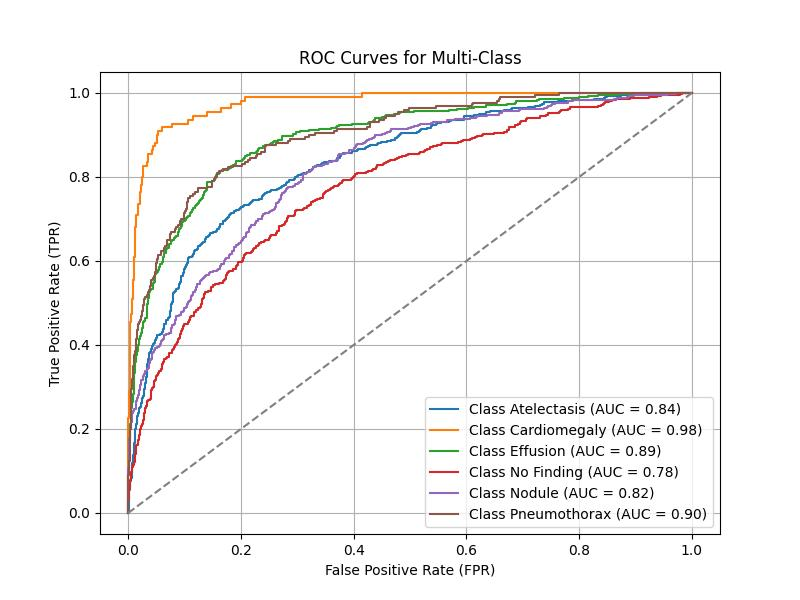
\includegraphics[width=0.54\textwidth]{roc_curve.png} % Replace with the actual path to your ROC curve image
    \caption{ROC-AUC Curve for the Classification Task. This curve demonstrates the model’s ability to distinguish between classes, with individual AUC values ranging from 0.78 (Class No Finding) to 0.98 (Class Cardiomegaly).}
    \label{fig:roc_curve}
\end{figure}

The tables and the ROC-AUC curve highlight the performance of our model. Despite a relatively modest overall accuracy (55\%), the high AUC scores, particularly for critical classes like Cardiomegaly (0.98) and Pneumothorax (0.90), demonstrate the potential for practical diagnostic applications. Addressing sensitivity and specificity imbalances, especially in underrepresented classes, remains crucial for further improving model performance.

\section{Code Explanation}

In this section, we provide a detailed explanation of the code used in the project. The code is divided into several key sections: data preparation, model creation, model compilation, callbacks, and training. Below is a detailed description of each part.

\subsection{Data Preparation and Augmentation}

The first step in the code involves importing necessary libraries and setting up data generators for both the training and validation datasets.

\begin{itemize}
    \item \texttt{train\_datagen} and \texttt{val\_datagen} are instances of \texttt{ImageDataGenerator} used to perform data augmentation on the training dataset and normalization on the validation dataset \cite{github-nih-chest-xrays}. For the training set, random transformations such as rotation, width and height shifts, shear, and zoom are applied to make the model robust and prevent overfitting.
    \item \texttt{train\_generator} and \texttt{val\_generator} are used to load images from the specified directories, resize them to the target image size (\texttt{IMAGE\_SIZE}), and generate batches of data. The images are scaled by a factor of 1/255 to normalize the pixel values to a range of [0, 1].
\end{itemize}

\subsection{Class Weights Calculation}

The dataset might be imbalanced, meaning some classes may have fewer samples than others. To handle this, class weights are calculated using \texttt{compute\_class\_weight} from \texttt{sklearn.utils}. The computed weights are then converted into a dictionary for use during training. This ensures that the model gives more attention to underrepresented classes.

\subsection{Model Creation with ResNet50}

The model is built by first loading the pre-trained ResNet50 model without the top layers (i.e., excluding the fully connected layers), which are not needed for our classification task. This pre-trained model is used as a feature extractor.

\begin{itemize}
    \item \texttt{base\_model} is initialized with the pre-trained weights from ImageNet. The input shape is set to (224, 224, 3), as required by the ResNet50 model. \texttt{include\_top=False} ensures that the fully connected layers of ResNet50 are excluded.
    \item The output of the base model is passed through a \texttt{GlobalAveragePooling2D} layer, which reduces the spatial dimensions of the feature maps.
    \item A \texttt{Dropout} layer with a rate of 0.5 is added to regularize the model and prevent overfitting.
    \item A \texttt{Dense} layer with softmax activation is added at the output, which is responsible for classifying the input into one of the six classes\cite{prof-koc}.
\end{itemize}

\subsection{Model Compilation}

The model is compiled using the Adam optimizer, which is a popular choice for training deep neural networks. The loss function used is \texttt{CategoricalCrossentropy} with label smoothing set to 0.1 to help improve model generalization. The performance of the model is evaluated using the accuracy metric and the AUC (Area Under the Curve) metric.

\subsection{Callbacks}

Several callbacks are used to improve training and model performance:

\begin{itemize}
    \item \texttt{ModelCheckpoint} saves the best model based on validation accuracy during training.
    \item \texttt{EarlyStopping} monitors the validation accuracy and stops training if the accuracy does not improve for 10 consecutive epochs, helping to avoid overfitting.
    \item \texttt{ReduceLROnPlateau} reduces the learning rate by a factor of 0.5 if the validation loss plateaus, helping the model to converge more effectively.
\end{itemize}

\subsection{Training the Model}

The model is trained using the \texttt{fit} function, which takes the training and validation data generators, the number of epochs, class weights, and the defined callbacks as inputs. The model will be trained for a maximum of 30 epochs.

\subsection{Model Evaluation}

After training, the model is evaluated on the validation data using the \texttt{evaluate} method. This provides the final accuracy and loss metrics, which help assess how well the model generalizes to unseen data \cite{google-drive}.

\section{Personal Contributions}

\begin{itemize}
    \item \textbf{Emre Dumbo}: Emre used his connections to a doctor and a machine learning specialist professor for valuable insights and collaboration. He contributed to code writing and debugging, code optimization, methodology research, and evaluation. Emre was also responsible for dataset selection and contributed a personal chest X-ray as a "no finding" test image to the dataset.
    
    \item \textbf{Bu\u{g}ra Muh\c{c}i}: Bu\u{g}ra connected with a friend who is a doctor for assistance with class selection from the dataset. He was involved in code writing and debugging, code optimization, prompt engineering, data preprocessing, and model evaluation and selection.
\end{itemize}

\section{Discussion and Conclusion}

In this project, we classified lung diseases from chest X-ray images using deep learning models, specifically ResNet50. Several key observations were made:

\subsection{Model Performance}
The ResNet50 model achieved a validation accuracy of 55\%. While this result highlights the complexity of medical image classification tasks, the high AUC scores for critical classes such as Cardiomegaly (0.98) and Pneumothorax (0.90) demonstrate the potential for practical applications. Hyperparameter tuning revealed notable variability, with some configurations yielding perfect training accuracy (e.g., 100\%) but significantly lower validation accuracy (e.g., 50\%), pointing to challenges in generalization. While significant efforts were made to address sensitivity and specificity imbalances for underrepresented classes, these improvements were limited, indicating a need for further exploration in future work.

\subsection{Data Preprocessing and Augmentation}
Preprocessing steps, including normalization, rescaling, and data augmentation (e.g., rotations, shift), enhanced the model's generalization ability and mitigated overfitting. These techniques accounted for variations in chest X-ray images and were crucial to achieving stable performance.

\subsection{Handling Class Imbalance}
Class weighting effectively addressed class imbalance, ensuring the model did not favor more frequent classes. This strategy improved performance for underrepresented categories, showcasing its importance in medical datasets.

\subsection{Model Selection and Tuning}
The ResNet50 architecture was selected for its robust feature extraction capabilities. Fine-tuning, including label smoothing and dynamic learning rate adjustments, improved generalization. However, experiments with various hyperparameter settings demonstrated inconsistent outcomes, occasionally achieving overly high training accuracy with poor validation performance, reflecting a need for more stable optimization strategies. Despite our efforts to explore alternative architectures and hybrid models, performance improvements were incremental, suggesting further research is needed in this area.

\subsection{Future Directions}
To improve results, future work could focus on:
\begin{itemize}
\item Expanding the dataset size to include more diverse and balanced samples.
\item Refining hyperparameter tuning strategies to improve generalization stability and reduce overfitting.
\item Exploring advanced techniques such as domain-specific data augmentation, synthetic data generation, or self-supervised pretraining to enhance performance with limited data.
\end{itemize}

\subsection{Conclusion}
This project demonstrates the potential of deep learning in medical image analysis, showing promising results in identifying critical conditions. However, challenges such as dataset size, class imbalance, and generalization stability remain significant hurdles. The results underscore the need for continuous advancements in data quality, model design, and fine-tuning techniques to improve performance. Future work should focus on expanding datasets, refining model architectures, and exploring domain-specific pre-training to enhance the applicability of deep learning models in real-world healthcare settings.


\section{Ethical Statement}
We confirm that all experimental work in this project was carried out by us with integrity. All sources and methods used in the study have been properly cited and included in the references. No plagiarism has been committed in any part of this study.
\section{AI Tools Usage}

In this project, the main AI tool used was ChatGPT\cite{chatgpt}, which provided assistance in various aspects of the work. Specifically, the AI tool was used for:

\subsection{Code Writing and Debugging} ChatGPT helped generate code snippets, suggest optimizations, and offered solutions to issues encountered during development. This contributed to speeding up thze coding process and improving code quality.
    
\subsection{Code Optimization} The model provided suggestions for optimizing the code, including adjusting certain parameters and refining the implementation to improve performance and efficiency.


\subsection{Methodology Clarifications} Whenever clarification was needed on methodology or machine learning concepts, ChatGPT provided concise explanations, helping to ensure that the project’s approach was well-understood and properly framed.

Although ChatGPT assisted in various technical and writing-related tasks, it is important to note that the conceptual work, data collection, model selection, and decision-making were entirely handled by the team. The contributions of ChatGPT were meant to support the team’s efforts and enhance the overall quality of the project, but the primary responsibility for the work lies with the team members. 

\begin{thebibliography}{99}

\bibitem{nih-chest-xrays} 
Kaggle, "NIH Chest X-rays Dataset," \url{https://www.kaggle.com/datasets/nih-chest-xrays/data}, [Accessed: Dec. 2024].

\bibitem{chatgpt} 
OpenAI, "ChatGPT," \url{https://chat.openai.com}, [Accessed: Dec. 2024].

\bibitem{github-nih-chest-xrays} 
P. Loukari, "NIH Chest X-rays Classification," GitHub repository, \url{https://github.com/paloukari/NIH-Chest-X-rays-Classification/tree/master}, [Accessed: Dec. 2024].

\bibitem{keras-api}
Keras, "Keras API Documentation," \url{https://keras.io/api/}, [Accessed: Dec. 2024].

\bibitem{prof-koc} 
M. Koç, Associate Prof. Dr., Computer Science Branch, Department Chair, Eskişehir Technical University, Email: \url{mehmetkoc@eskisehir.edu.tr}.

\bibitem{prof-candemir} 
S. Candemir, Asst. Prof. Dr., Computer Science Branch, Department Vice Chair, Eskişehir Technical University, Email: \url{semacandemir@eskisehir.edu.tr}.

\bibitem{prof-karahoda} 
B. Karahoda, Associate Prof. Dr., Computer Science Branch, UBT Higher Education Institution.

\bibitem{med-student-koroglu} 
B. Köroğlu, Medical Student, Hacettepe University.

\bibitem{dr-kazazi} 
A. Kazazi, Assoc. Prof. Dr., Gazi University Faculty of Medicine.

\bibitem{tensorflow} 
TensorFlow, "TensorFlow API Documentation," \url{https://www.tensorflow.org/api_docs/python/tf}, [Accessed: Dec. 2024].

\bibitem{anaconda} 
Anaconda, Inc., "Anaconda Cloud," \url{https://anaconda.cloud}, [Accessed: Dec. 2024].

\bibitem{python} 
Python Software Foundation, "Python Documentation," \url{https://www.python.org/doc/}, [Accessed: Dec. 2024].

\bibitem{google-drive}
Google Drive, "ResNet50 Model and NIH Dataset," \url{https://drive.google.com/drive/folders/1DMyWrGlT2p1CiQlM6K2aXYlUdI-efoyM?usp=sharing}, [Accessed: Dec. 2024].


\end{thebibliography}

\end{document}
